
\documentclass[utf8]{article}
\usepackage[utf8]{inputenc}

\usepackage[parfill]{parskip}
\usepackage{booktabs}
\usepackage{amsmath}
\usepackage{amssymb}
\usepackage{amsfonts}
\usepackage{graphicx}
\usepackage{float}
\usepackage{listingsutf8}
\usepackage{listings}
\usepackage{graphicx}
\usepackage{hyperref}
\usepackage{fullpage}
\usepackage{lipsum}
\usepackage{multirow}

\nocite{*}
\setlength\parindent{24pt}

\begin{document}
\begin{titlepage}


  \author{Andrius Ezerskis \& Moïra Vanderslagmolen}
  \title{Projet d'Algorithmique: R-trees}
  \maketitle
\end{titlepage}
\tableofcontents
\newpage
\begin{large}



  dire quelles librairies on a utilisé


  \section{Introduction}
  \indent
  \par
  Ce rapport se divise en plusieurs parties. Tout d'abord, nous expliquons la
  structure de notre code en expliquant le rôle de chaque classe et leurs
  méthodes associées. Ensuite, nous parlerons des optimisations effectuées afin
  d'améliorer la vitesse de nos algorithmes. Enfin, nous analyserons les tests
  réalisés dans le cadre de ce projet et les influences des différentes
  optimisations sur le temps d'exécution.
  \par
  \section{Structure du code}

  \par
  \subsection{MBRNode}
  \indent
  \par
  MBRNode représente les noeuds des R-Tree. Elle contient un label, un Minimum Bouding Rectangle(MBR),un polygone,
  des enfants (sauf si c'est une feuille) et un parent (sauf si c'est la racine de
  l'arbre). Si le noeud n'est pas une feuille, alors son label sera `SplitSeed',
  et son MBR contiendra l'union de tous les MBR de ses enfants.
  \par

  \subsection{RTree}\label{RTree}
  \indent
  \par
  RTree est une classe abstraite. Elle permet de regrouper ensemble les méthodes
  communes à RTreeLinear et RTreeQuadratic, par exemple la recherche d'un noeud
  (searchNode), l'initialisation de la classe, les méthodes split, pickNext,
  chooseNode et addLeaf.
  \par

  \subsubsection{addLeaf}\label{addLeaf}
  \indent
  \par
  Lorsque nous voulons ajouter un nouveau node, la méthode addLeaf() est appelée
  avec la racine de l'arbre en paramètre. Si la racine de l'arbre n'a pas
  d'enfants ou que son premier enfant n'a pas d'enfant, alors le nouveau node
  est rajouté à la racine de l'arbre. Ensuite, nous augmentons le MBR du parent,
  ainsi que celui de ses parents grâce à la méthode expandMBR(). Sinon, nous
  choisissons un noeud grâce à la méthode \nameref{chooseNode} et puis la méthode \nameref{addLeaf}
  est de nouveau appelée, avec cette fois-ci le node choisi par la méthode
  \nameref{chooseNode}.
  \par
  \indent
  Si le nombre d'enfants du node passé en paramètre dépasse un nombre N, alors
  un split est effectué.
  \par
  \subsubsection{split}\label{split}
  \indent
  \par
  L'algorithme de split commence par appeler le pickSeeds quadratique ou
  linéaire afin d'obtenir deux seeds. \newline Ensuite, la
  méthode pickNext s'assure de choisir, pour chaque sous-noeud, la seed dont le
  MBR augmente le moins avec ce sous-noeud, et le sous-noeud devient alors
  l'enfant de cette seed. \newline Pour finir, les deux splitSeeds obtenus via
  pickSeeds reçoivent comme parent le node (celui que l'on doit split) et,
  réciproquement, le node reçoit les deux splitSeeds comme ses enfants. Le noeud
  a été divisé.
  \par

  \subsubsection{chooseNode}\label{chooseNode}
  \indent
  \par
  La méthode chooseNode prend en paramètre le bestNode et le noeud à ajouter.
  Si le bestNode n'a pas d'enfants ou si son premier enfant n'a pas d'enfants,
  alors le bestNode est renvoyé. Sinon, nous itérons à travers les enfants de
  bestNode. Le noeud dont le MBR augmente le moins avec le noeud à ajouter est
  choisi. Nous appelons ensuite récursivement la méthode chooseNode.

  \par
  \subsubsection{search}
  \indent
  \par


  \par
  \subsection{RTreeLinear et RTreeQuadratic}\label{RTreeLinear}
  \indent
  \par
  RTreeLinear représente l'implémentation du R-Tree avec l'algorithme de split
  linéaire, dont on reparle dans la section PickSeedsLinear. RTreeQuadratic
  représente donc le R-Tree avec l'algorithme de split quadratique.
  \par

  \subsubsection{PickSeeds quadratique}\label{PickSeeds quadratique}
  \indent
  \par
  Le pickSeeds quadratique cherche les deux seeds qui maximisent l'aire de l'enveloppe qui les entoure.
  \newline Pour ce faire, nous itérons à travers tous les sous-noeuds du noeud donné en paramètre,
  et nous calculons la différence d'aire entre l'union de deux sous-noeuds consécutifs et l'aire de
  ces derniers séparement (enveloppe(les 2 sous-noeuds) - enveloppe(premier sous-noeud) - enveloppe(deuxième sous-noeud)).
  \newline Le pickSeeds retourne donc un vecteur contenant les deux seeds choisies.
  \par
  \subsubsection{PickSeeds linéaire}\label{PickSeeds lineaire}
  \indent
  \par
  Le pickSeeds linéaire commence par itérer dans chaque sous-noeud du noeud
  qu'on veut split. Ensuite, nous choisissons le noeud dont le côté droit du MBR
  associé a le plus petit x, le noeud dont le côté gauche du MBR a le plus grand
  x. Nous faisons de même avec la dimension y. Par après, nous testons si les
  nodes sont tous les mêmes, ou si les noeuds d'une dimension sont les mêmes.
  Dans le premier cas, nous renvoyons null et le split ne se produit pas. En
  effet, si les seeds trouvées sont les mêmes, alors le split ne se produira pas
  correctement car tous les noeuds iront donc dans la première seed. Dans le
  deuxième cas, nous choisissons l'autre dimension dont les seeds ne sont pas
  les mêmes.
  \par
  \indent
  \par
  Si les noeuds sont tous différents, nous calculons la normalisation, qui
  correspond au ratio entre les côtés internes et les côtés externes pour chaque
  dimension(dans ce projet-ci, la dimension x et y). Nous prenons ensuite la
  normalisation la plus élevée.
  \par

  \subsection{FileLoader}
  \indent
  \par
  Cette classe permet de charger le shapefile en mémoire. Nous avons implémenté
  cette classe afin de facilement changer la façon dont les fichiers sont chargés.


  \section{Optimisations}
  \subsection{Multi-polygones}
  \indent
  \par
  Notre première optimisation se base sur les multi-polygones. En effet, comme
  expliqué dans les consignes du projet d'algorithmique, nous avons remarqué que
  des polygones très étendu comme la france (voir annexe, mettre un label)
  prenaient énormément de place. Nous avons donc décidé de séparer les
  multi-polygones en polygones et ça a donné (figure aprèsopti). Cela nous a
  permis de gagner quelques secondes lors des tests dont nous parlerons au
  chapitre 'Analyse des tests'.

  \subsection{Split}
  \indent

  \par
  Au début, nous copions l'entiereté du vecteur des enfants du node choisi pour
  split. Puis nous vidons ce vecteur et nous rajoutons les seeds choisies. Et puis
  seulement avec le vecteur copié nous ajoutions au fur et à mesure au seeds
  choisies. Nous nous sommes dit qu'on perdait bcp de temps à copier l'entiereté
  du vecteur, surtout sur des gros vecteurs.

  Nous avons donc changé l'ordre, d'abord nous appelons pickNext pour qu'il
  rajoute les enfants aux seeds, puis nous vidons le vecteur du node à spliter et
  rajoutons les splits seeds.

  Grâce à cette amélioration, les 8 tests que nous avons fait tourner ont pris
  5,865 secondes au total au lieu de 6,778 secondes.
  \par
  \subsection{PickSeeds quadratique}
  \indent
  \par
  Dans le pickSeeds quadratique, nous itérons à travers le vecteur d'enfants du node à
  split et nous prenons les deux noeuds les plus éloignés. Nous avons vite
  remarqué qu'il n'était pas nécéssaire de faire un double for en itérant chaque
  élément dans le vecteur. En effet, si nous calculons l'aire pour le noeud A
  et pour le noeud B, il ne faut pas recalculer pour le noeud B et le noeud A, de
  même qu'il ne faut pas calculer l'aire pour le noeud A et le noeud A. Nous
  faisons donc deux boucles for, l'une itérant dans le vecteur entier de
  sous-noeuds, l'autre commençant à l'indice de la précédente boucle + 1. De cette
  manière, nous commençons avec le noeud A et calculons avec le noeud B et tous
  les autres noeuds restants, puis le noeud B avec le noeud C et ainsi de suite. Cela nous permet de réduire le temps d'exécution.

  \subsection{N}
  \indent
  \par
  Au début, nous avions N, le truc maximum pr les RTree en attribut de la classe RTree et défini là dedans.
  Pour optimiser notre programme, nous avons décidé de le passer en paramètre.
  Grâce à cette amélioration, les 8 tests que nous avons fait tourner ont pris
  4,429 secondes au total au lieu de 5,865 secondes.


  \section{Expérience sur données réelles}
  \subsection{Présentation des tests}
  \begin{enumerate}
    \item Carte de la belgique - Algorithme linéaire - Campus universitaire
    \item Carte de la belgique - Algorithme linéaire - Point pas dans le polygone
    \item Carte du monde - Algorithme linéaire - Kazakhstan
    \item Carte du monde - Algorithme linéaire - Canada
    \item Carte de la france - Algorithme linéaire - Auvergne
    \item Carte de la france - Algorithme linéaire - Guyane
    \item Carte de la belgique - Algorithme quadratique - Campus universitaire
    \item Carte de la belgique - Algorithme quadratique - Point pas dans le polygone
    \item Carte du monde - Algorithme quadratique - Kazakhstan
    \item Carte du monde - Algorithme quadratique - Canada
    \item Carte de la france - Algorithme quadratique - Auvergne
    \item Carte de la france - Algorithme quadratique - Guyane
  \end{enumerate}

  \subsection{Présentation des cartes}
  \begin{enumerate}
    \item Carte de la belgique : 19795 polygones
    \item Carte du monde : 251 polygones
    \item Carte de la france : 18 polygones
  \end{enumerate}

  \indent
  \par
  Ces tests ont été effectués sur une machine Lenovo Yoga 7. La distribution
  linux est KDE Neon 5.27 et la release ubuntu est la 22.04.
  \indent

  \subsection{Résultats des tests}
  \indent
  \par
  Temps en millisecondes de la fonction search en fonction des différents tests et valeurs.

  \begin{tabular}{ |p{3cm}||p{3cm}|p{3cm}|p{3cm}|  }
    \hline
    \multicolumn{4}{|c|}{Temps en millisecondes de la fonction search} \\
    \hline
    Test   & N=4 & N = 500 & N = 10000                                 \\
    \hline
    Test1  & 15  & 15      & 17                                        \\
    Test2  & 1   & 1       & 1                                         \\
    Test3  & 76  & 8       & 11                                        \\
    Test4  & 123 & 214     & 219                                       \\
    Test5  & 23  & 68      & -                                         \\
    Test6  & 3   & 3       & -                                         \\
    Test7  & 2   & 0       & 2                                         \\
    Test8  & 1   & 1       & 4                                         \\
    Test9  & 3   & 2       & 2                                         \\
    Test10 & 29  & 76      & 73                                        \\
    Test11 & 29  & 37      & -                                         \\
    Test12 & 2   & 2       & -                                         \\
    \hline
  \end{tabular}

  \begin{tabular}{ |p{3cm}||p{3cm}|p{3cm}|p{3cm}|  }
    \hline
    \multicolumn{4}{|c|}{Temps en millisecondes de la fonction search avec l'optimisation} \\
    \hline
    Test   & N=4 & N = 500 & N = 10000                                                     \\
    \hline
    Test1  & 12  & 14      & 19                                                            \\
    Test2  & 1   & 1       & 6                                                             \\
    Test3  & 11  & 12      & 9                                                             \\
    Test4  & 20  & 28      & 23                                                            \\
    Test5  & 99  & 95      & -                                                             \\
    Test6  & 3   & 2       & -                                                             \\
    Test7  & 3   & 0       & 2                                                             \\
    Test8  & 0   & 3       & 2                                                             \\
    Test9  & 1   & 2       & 2                                                             \\
    Test10 & 5   & 5       & 6                                                             \\
    Test11 & 29  & 19      & -                                                             \\
    Test12 & 2   & 2       & -                                                             \\
    \hline
  \end{tabular}



  \subsection{Analyse des données}
  \subsubsection{Optimisation}
  \par
  \indent
  Nous avons donc remarqué suite à cela que le test 4 prenait beaucoup de temps,
  et plus généralement les tests concernant la carte du monde (Test 3, 4, 9, 10)
  et les tests concernant la carte de la france (Test 5,6,11,12). Ces tests
  devraient être les plus rapides, car ils contiennent le moins de polygones, et
  les algorithmes sont quadratiques et linéaire. Nous avons compris que le
  problème venait du fait que les multi-polygones prenait énormément de place et nous avons refait les tests
  \subsubsection{Influence du N}
  Nous remarquons aussi que le
  nombre N n'a pas d'influence sur la rapidité de notre algorithme.
  \subsubsection{Algorithme linéaire vs Algorithme quadratique}
  \par
  \indent
  Nous avons aussi remarqué que l'algorithme linéaire prend beaucoup plus de temps
  à chercher un point dans un polygone. En moyenne, la recherche prend 39,9
  millisecondes pour l'algorithme linéaire et 13,25 millisecondes pour
  l'algorithme quadratique. Nous avons donc comparé les temps d'exécution. En
  moyenne, le temps d'exécution sur 6 tests pour l'algorithme quadratique est de
  6,357 secondes. Le temps d'exécution sur les mêmes tests pour l'algorithme
  linéaire est de 3,087 secondes. La création de l'arbre est donc beaucoup plus
  rapide pour l'algorithme linéaire que pour le quadratique, ce qui est attendu vu
  la complexité de chaque algorithme. Cependant, il est intéressant de noter que
  la fonction de recherche prend beaucoup plus de temps dans l'algorithme
  linéaire.
  \par

  \section{Conclusion}
  \indent
  \par
  \par

  \section{Bibliographie}

  \section{Annexes}
  \begin{figure}[h]
    \caption{Before optimization}
    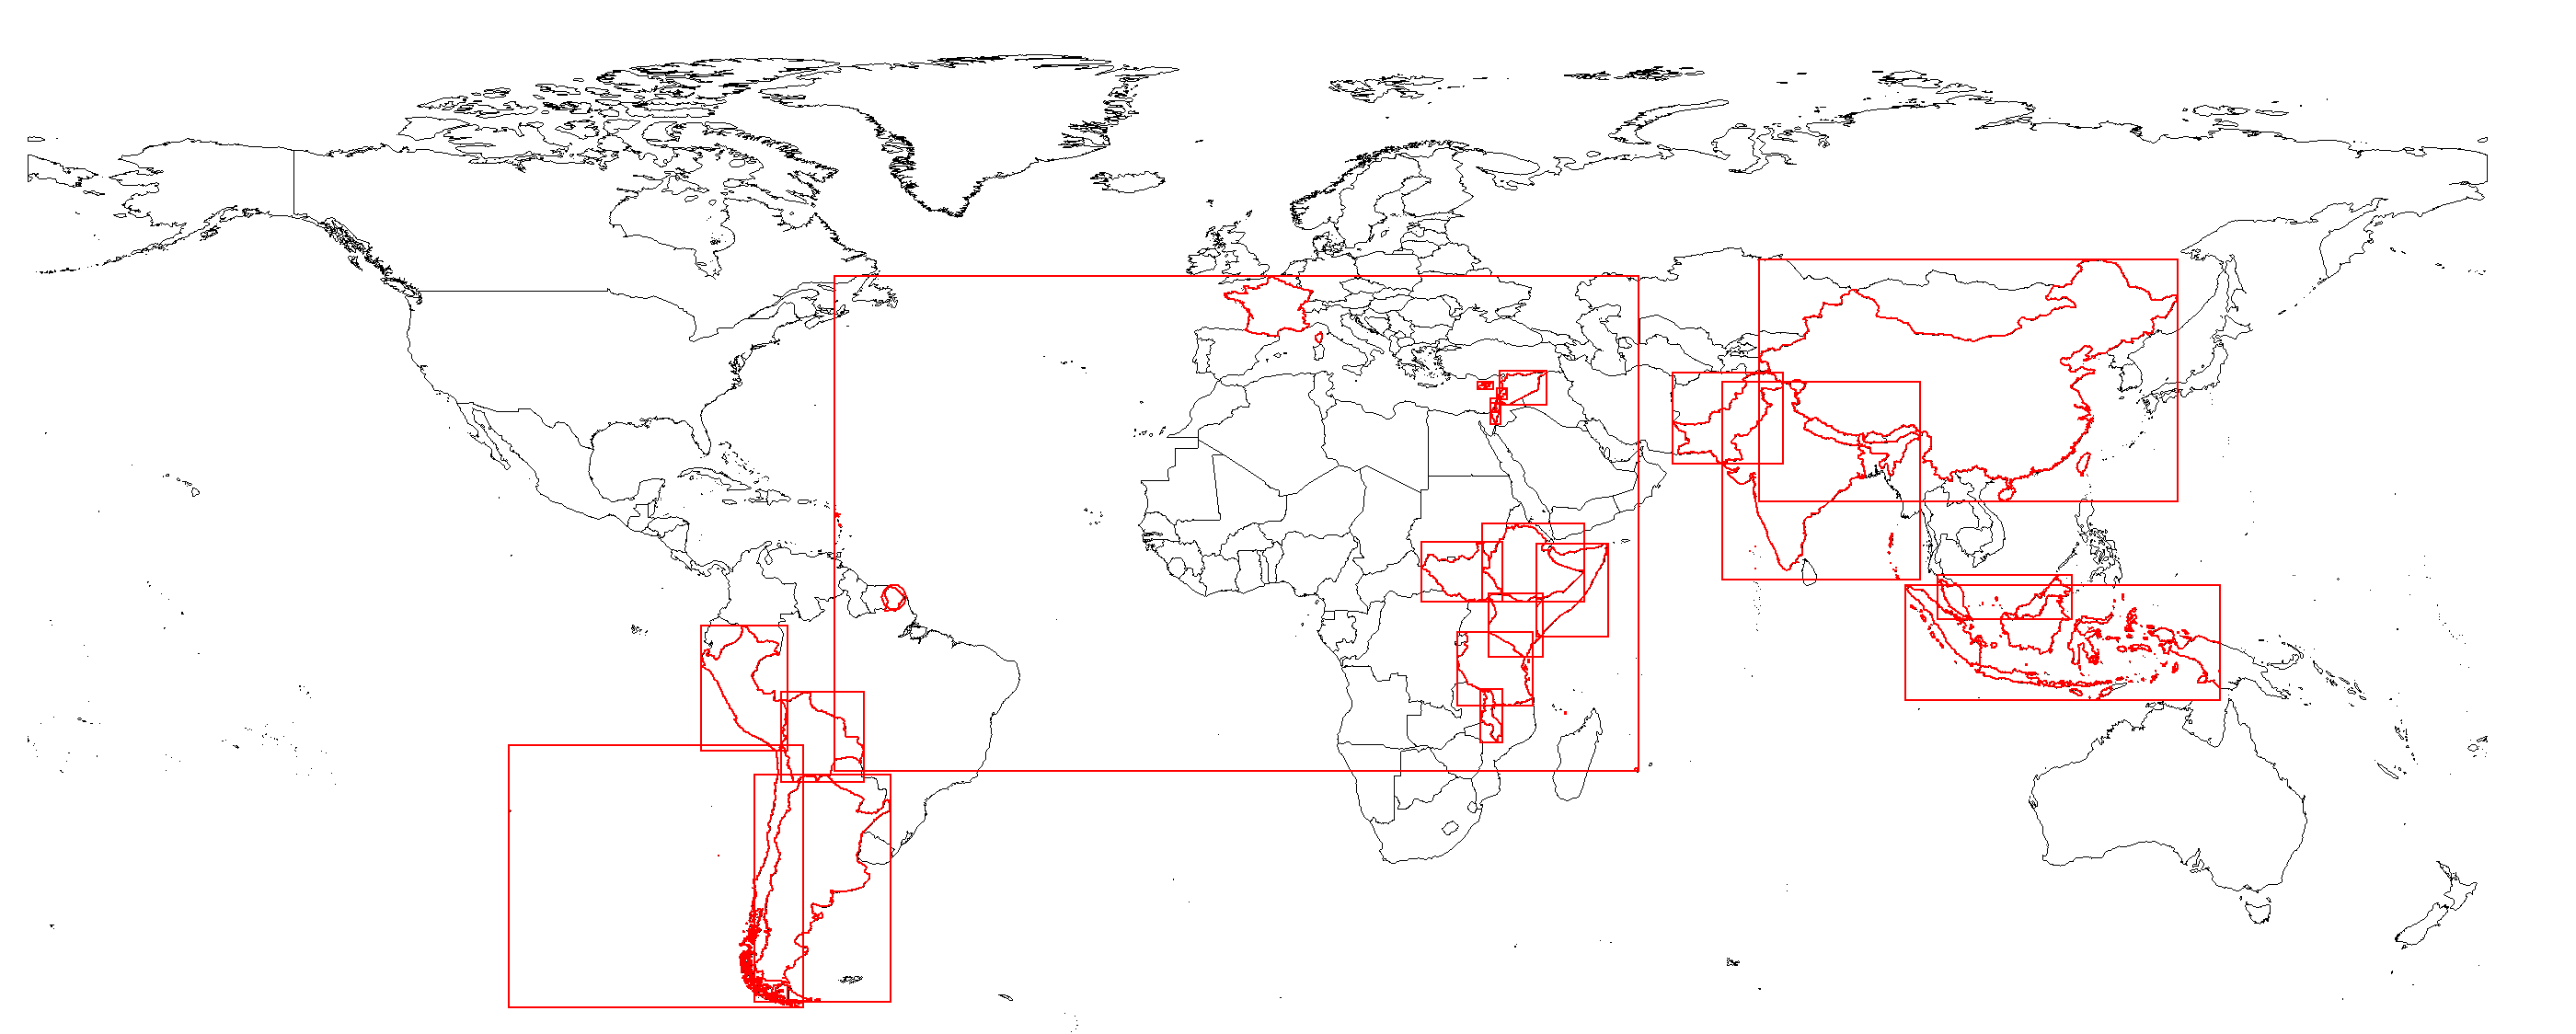
\includegraphics[width=\textwidth]{beforeopti.png}\label{fig:beforeopti}
  \end{figure}

  \begin{figure}[h]
    \caption{After optimization}
    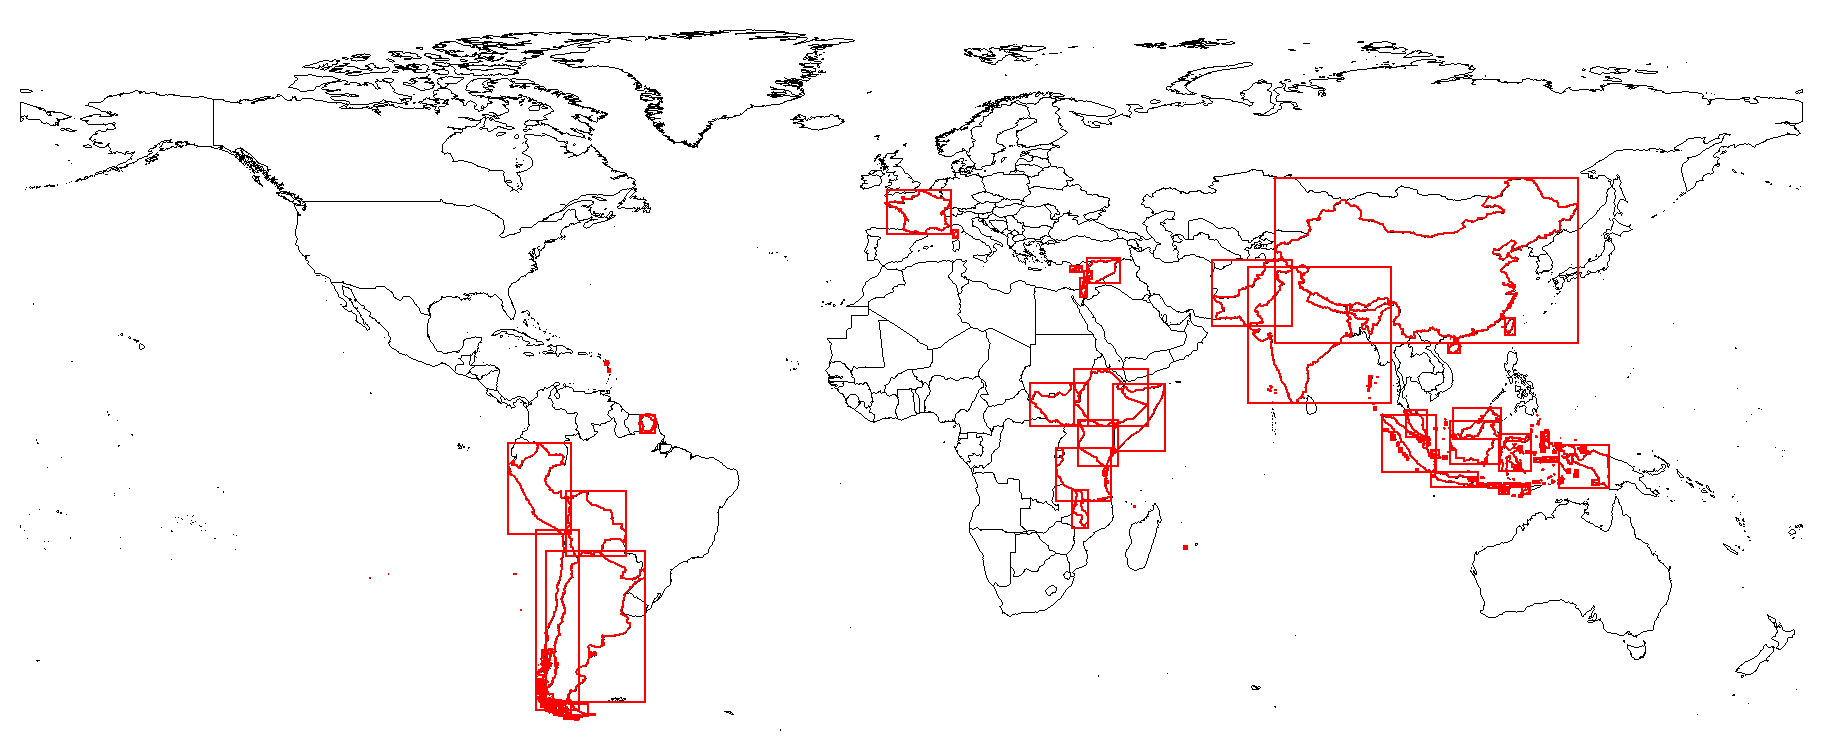
\includegraphics[width=\textwidth]{afterOpti.png}\label{fig:afteropti}
  \end{figure}


\end{large}

\end{document}
